\documentclass[
  % -- opções da classe memoir --
  12pt,				% tamanho da fonte
  %openright,			% capítulos começam em pág ímpar (insere página vazia caso preciso)
  openany,
  %twoside,			% para impressão em verso e anverso. Oposto a oneside
  oneside,
  %titlepage,
  a4paper,			% tamanho do papel.
  % -- opções da classe abntex2 --
  %chapter=TITLE,		% títulos de capítulos convertidos em letras maiúsculas
  %section=TITLE,		% títulos de seções convertidos em letras maiúsculas
  %subsection=TITLE,	% títulos de subseções convertidos em letras maiúsculas
  %subsubsection=TITLE,% títulos de subsubseções convertidos em letras maiúsculas
  % -- opções do pacote babel --
  english,			% idioma adicional para hifenização
  brazil
]{article}
\usepackage[utf8]{inputenc}
\usepackage[brazil]{babel}
\usepackage{amsfonts}
\usepackage{indentfirst}
\usepackage[T1]{fontenc}
\usepackage{helvet}
\renewcommand{\familydefault}{\sfdefault}
\usepackage[left=3cm, right=2cm, top=3cm, bottom=2cm]{geometry}
\usepackage{setspace}
\usepackage{epigraph}
\usepackage{graphicx}
\usepackage{hyperref}
\usepackage{amsmath}
\numberwithin{figure}{section}
\numberwithin{table}{section}

%\usepackage{biblatex}
%\bibliography{relEstagio1}

\graphicspath{{figuras/}}

\renewcommand{\baselinestretch}{1.5}
\setlength{\parindent}{3em}
\setlength{\parskip}{1em}

%% DEFINEs dos textos constantes da capa
\newcommand{\defUFABC}{UNIVERSIDADE FEDERAL DO ABC}
\newcommand{\defBCC}{BACHARELADO EM CIÊNCIA DA COMPUTAÇÃO}
\newcommand{\defRelatorio}{RELATÓRIO DO ESTÁGIO SUPERVISIONADO I} %%ESTÁGIO SUPERVISIONADO
\newcommand{\defTitulo}{ESTÁGIO EM DESENVOLVIMENTO DE SISTEMA PARA USO INTERNO NA AGÊNCIA CADARIS}
\newcommand{\defRafael}{RAFAEL CARDOSO DA SILVA}
\newcommand{\defOrientador}{Orientador: Prof. Dr. Daniel Morgato Martin}
\newcommand{\defLocaldata}{Santo André, 2017}

%%%%% \subsubsubsection
\usepackage{titlesec}
\usepackage{hyperref}
\titleclass{\subsubsubsection}{straight}[\subsection]

\newcounter{subsubsubsection}[subsubsection]
\renewcommand\thesubsubsubsection{\thesubsubsection.\arabic{subsubsubsection}}
\renewcommand\theparagraph{\thesubsubsubsection.\arabic{paragraph}} % optional; useful if paragraphs are to be numbered

\titleformat{\subsubsubsection}
{\normalfont\normalsize\bfseries}{\thesubsubsubsection}{1em}{}
\titlespacing*{\subsubsubsection}
{0pt}{3.25ex plus 1ex minus .2ex}{1.5ex plus .2ex}

\makeatletter
\renewcommand\paragraph{\@startsection{paragraph}{5}{\z@}%
  {3.25ex \@plus1ex \@minus.2ex}%
  {-1em}%
  {\normalfont\normalsize\bfseries}}
\renewcommand\subparagraph{\@startsection{subparagraph}{6}{\parindent}%
  {3.25ex \@plus1ex \@minus .2ex}%
  {-1em}%
  {\normalfont\normalsize\bfseries}}
\def\toclevel@subsubsubsection{4}
\def\toclevel@paragraph{5}
\def\toclevel@paragraph{6}
\def\l@subsubsubsection{\@dottedtocline{4}{7em}{4em}}
\def\l@paragraph{\@dottedtocline{5}{10em}{5em}}
\def\l@subparagraph{\@dottedtocline{6}{14em}{6em}}
\makeatother

\setcounter{secnumdepth}{4}
\setcounter{tocdepth}{4}



\begin{document}

%%--[ELEMENTOS PRÉ-TEXTUAIS]--%%

%%--CAPA--%%

\begin{titlepage}

\begin{center}
\text{ \defUFABC }
\text{ \defBCC }\\\vspace{5cm}
\textbf{\large{ \defRelatorio }}\\\vspace{4cm}
\textbf{\Large{\defTitulo}}\\\vspace{4cm}
% Nome do Autor
\textbf{\large{ \defRafael }}\\\vspace{2cm}
% Orientador
\textbf{\large{ \defOrientador }}\\\vspace{3cm}
\textbf{\defLocaldata}
\end{center}

\end{titlepage}

%%--FOLHA DE ROSTO--%%

\begin{titlepage}

\begin{center}
\textbf{\large{ \defRafael }}\\\vspace{6cm}
\textbf{\Large{ \defTitulo }}\\\vspace{5cm}
\begin{raggedleft}{
Relatório do Estágio apresentado ao Curso de\\
Bacharelado em Ciência da Computação como\\
requisito parcial para obtenção do grau de\\
Bacharel em Ciência da Computação
\\\vspace{1cm}

%  Trabalho apresentado à banca de Estágio\\
%  Supervisionado como requisito parcial para\\
%  obtenção do título de Bacharel em Ciência da\\
%  Computação pela Universidade Federal do ABC.\\
\large{ \defOrientador }
}\\\vspace{5cm}
\end{raggedleft}
\textbf{ \defLocaldata }
\end{center}

\end{titlepage}

%%--DEDICATÓRIA--%%

\begin{titlepage}

\begin{center}
\textbf{DEDICATÓRIA}
\end{center}

Dedico todo projeto realizado aos meus amigos e familiares que depositaram grande confiança em mim desde o início.


\end{titlepage}

%%--AGRADECIMENTOS--%%

\begin{titlepage}

\begin{center}
\textbf{AGRADECIMENTOS}
\end{center}

Meus agradecimentos são voltados à agência Cadaris, principalmente a Diretora Comercial, que propôs essa oportunidade de amadurecer meus conhecimentos obtidos na Universidade Federal do ABC, além do crescimento pessoal.


\end{titlepage}

%%--EPÍGRAFE--%%

%\begin{titlepage}
%.\\\vspace{18cm}
%\begin{raggedleft}
%
%\begin{epigraph} {????????????????????? \\A maioria das pessoas pensa no sucesso e no fracasso como opostos, mas eles são ambos produtos do mesmo processo}{Roger Von Oech}
%
%\end{epigraph}
%\end{raggedleft}
%
%\end{titlepage}

%%--RESUMO--%%

\begin{titlepage}

\begin{center}
\textbf{RESUMO}
\end{center}

Este estágio consiste no desenvolvimento completo de um sistema ERP (Planejamento dos Recursos da Empresa), da Proposta Comercial e de outros processos administrativos, para a empresa Cadaris Comunicação. Pois, o sistema atual contratado é ineficiente, havendo a necessidade do desenvolvimento de um novo sistema exclusivo que possa suportar os novos moldes da empresa, a fim de substituir esta ferramenta defasada. O novo sistema será desenvolvido em PHP em conjunto com o \textit{framework} Laravel. O estágio se inicia com reuniões, com a intenção de apresentar todas as regras de negócio da empresa e projetar o novo sistema para apoiar os processos administrativos. Logo após, há o estudo necessário para realizar a implementação do sistema. E ao final, o desenvolvimento de uma melhor interface com o proposito de favorecer a experiência do usuário.

% TODO: RESUMO revisar

\end{titlepage}

%%--ABSTRACT--%%

%\begin{titlepage}
%
%\begin{center}
%\textbf{ABSTRACT}
%\end{center}
%% TODO: RESUMO ingles
%
%????????????????? DEPOIS ?????????????????
%
%%The internship is the maintenance of existing systems in PHP, both on user access permissions as information security. Usually fixes and adding information to existing functionality. New systems are developed with the .NET framework, SQL Server database and MVC pattern. To enhance the experience of development and user, modern tools are explored, such as angularjs by Google. The scholarship system was the first with the tool and, after successful development and testing, started the project management system with maximum exploitation of resources, more quickly and standard development and a more active and dynamic experience by the user.
%
%
%\end{titlepage}


%%--LISTA DE FIGURAS--%%

\begin{titlepage}

\begin{singlespace}
  \listoffigures
\end{singlespace}

\end{titlepage}


%%--SUMÁRIO--%%

\begin{titlepage}

\begin{singlespace}
  \tableofcontents
\end{singlespace}

\end{titlepage}


%%--[ELEMENTOS TEXTUAIS]--%%

\section{INTRODUÇÃO}

O estágio é uma atividade fundamental para a formação do aluno que está matriculado em um curso de nível superior, já que o discente tem a possibilidade de fazer uma aliança entre os conhecimentos adquiridos durante o período de graduação com a experiência vivencial no ambiente corporativo. 

Além de agregar a responsabilidade de ter uma profissão, o estágio permite que o aluno desenvolva habilidades que são essenciais no mercado de trabalho, tais como liderança, trabalhar em equipe, resiliência, entre outros, através de situações e desafios que possam vir ocorrer dentro da organização e de suas responsabilidades.

O estágio é uma tarefa supervisionada por um orientador, e a descrição e avaliação do aluno quanto às suas atividades, conhecimentos adquiridos e habilidades desenvolvidas são relatados em um relatório.

Este relatório tem por objetivo descrever as atividades e os produtos obtidos durante a disciplina de Estágio Supervisionado I. Nesta seção, apresenta-se a caracterização do estágio, da empresa, uma visão geral do estágio e a organização geral deste documento.



\subsection{CARACTERÍSTICAS DO ESTÁGIO}

A modalidade deste estágio é em \textit{Home Office}\footnote{Escritório em casa, em uma tradução livre do inglês, trabalho que é realizado em espaço alternativo ao escritório de uma empresa.}, que também pode ser definido com um trabalho remoto ou teletrabalho, para a Cadaris Comunicação~\cite{cadaris}. A jornada de trabalho é de segunda à sexta-feira, desempenhando 6 horas diárias, totalizando 30 horas semanais, com a gratificação de uma bolsa de R\$ 1.100,00 por mês.

Por se tratar de um \textit{Home Office}, proporcionou ao discente um horário flexível de trabalho fazendo com que ele tenha autonomia para conciliar seu trabalho com as suas outras atividades. A comunicação com a empresa foi mantida através de e-mails e ligações via telefone e \textit{Skype}.

O objetivo geral deste estágio é o desenvolvimento de um projeto de uso interno para a empresa.




\subsection{CARACTERIZAÇÃO E ANÁLISE DA EMPRESA}

%  A Cadaris é uma agência de publicidade com atuação nas áreas de marketing, editorial e comunicação. Aqui, trabalho em equipe é lei e surpreender o cliente, uma meta diária.
%  Trabalhamos com ética e transparência, de forma responsável e comprometida. Produzimos com qualidade e criatividade, sempre com respeito aos prazos acordados.
%  Queremos ser reconhecidos como uma agência diferenciada, por clientes e funcionários.
%  Entre os nossos principais clientes estão: Colgate-Palmolive, Biotropic, ABO, TAM e Mattel, entre outras empresas.
%  Para saber mais sobre a Cadaris, acesse www.cadaris.com.br ou envie um email para cadaris@cadaris.com.br

%  Products:
%    Publicidade: anúncios, materiais de ponto de venda, materiais promocionais, apresentações de produtos e campanhas, hotsites, etc.
%    Comunicação: campanhas dirigidas e campanhas de comunicação interna
%    Editorial: revistas, informativos, enews, jornal-mural, guias e relatórios, manuais, cartilhas, etc.
%  ONDE A GENTE ATUA
%  EDITORIAL
%    Desenvolvimento de conteúdos editoriais baseado em planejamento, organização e processos de jornalismo.
%  ESTRATÉGIA
%    Criação de campanhas e peças de comunicação dirigida, comunicação interna, incentivo de vendas e marketing de relacionamento.
%  PUBLICIDADE
%    Assertividade em briefing, agilidade e criatividade são os drivers na criação das peças publicitárias e promocionais.
%  WEB
%    Levantamento de requisitos e necessidades, arquitetura da informação, design de projeto e desenvolvimento web.


O estágio foi iniciado no dia 01 de Agosto de 2016, contratado pela Cadaris Comunicações, CNPJ 01.556.009/0001-46, que é uma agência de publicidade e está localizada na R. Dr. Thirso Martins, 100, cj 303, CEP:~04120-050, Vila Mariana, São Paulo~-~SP, telefone:~(11)~5571-9142.

Fundada em 11 de novembro de 1996, pelos sócios Maristela Harada e Frederico Pimenta, a Cadaris Comunicação é formada por profissionais de diferentes áreas da comunicação, o que proporciona mais eficácia e agilidade. Trabalhando com ética e transparência, de forma responsável e comprometida. Produzindo com qualidade e criatividade, sempre com respeito aos prazos acordados.

A Cadaris é uma agência de comunicação com atuação nas áreas de:
\vspace{-0.5cm}

\begin{description}
   \item [EDITORIAL] Desenvolvimento de conteúdos editoriais baseado em planejamento, organização e processos de jornalismo, como produtos: revistas, informativos, enews, jornal-mural, guias e relatórios, manuais, cartilhas, etc.
   \item [ESTRATÉGIA] Criação de campanhas e peças de comunicação dirigida, comunicação interna, incentivo de vendas e marketing de relacionamento.
   \item [PUBLICIDADE]  Assertividade em briefing, agilidade e criatividade, produzindo: Anúncios, materiais de ponto de venda, materiais promocionais, apresentações de produtos e campanhas, hotsites, etc.
   \item [WEB] Levantamento de requisitos e necessidades, arquitetura da informação, design de projeto e desenvolvimento web.
\end{description}

Entre os principais clientes da Cadaris estão: Colgate-Palmolive, Biotropic, ABO, TAM e Mattel.


\subsection{VISÃO GERAL DO ESTÁGIO}


Durante o primeiro mês, o estagiário foi introduzido ao funcionamento da agência com a familiarização das regras do negócio e foram apresentadas as ferramentas atuais utilizadas para apoiar a administração da empresa. A fim de desenvolver um \textit{software} de Sistema de Gestão Empresarial substituto, para uso interno da Cadaris.

Após este período, foi feito o estudo das tecnologias que seriam utilizadas para o desenvolvimento deste sistema proposto que já estavam sendo discutidas desde o início do estágio.

Em seguida, iniciou-se a implementação do sistema com foco inicial no \textit{Back-end} que foram seguidas em três etapas: Desenvolvimento do Cadastro de Recursos e algumas rotinas administrativas; Processo Comercial; Geração de Relatórios e Controle Financeiro.

Por fim, foi desenvolvido um \textit{Front-end} definitivo para o sistema, junto ao time de \textit{Front-end} da Cadaris, com todos os recursos necessários para uma melhor experiência do usuário.



%\subsection{ORGANIZAÇÃO DESTE RELATÓRIO} %% {ORGANIZAÇÃODO TRABALHO}
%
%As próximas seções estão organizadas como segue:
%
%A seção 2 apresenta as informações detalhadas de todas as atividades realizadas pelo estagiário. A seção está dividida em quatro partes, uma para cada atividade desenvolvida.
%
%A seção 3 descreve as considerações finais em relação a todo o estágio, como: contribuições para a formação, dificuldades encontradas e sugestões para trabalhos futuros.
%
%A seção 4 apresenta os principais problemas observados pelo estagiário em cada etapa e sugestões de melhorias para cada uma delas.
%
%A seção 5 detalha a relação entre as disciplinas cursadas pelo estagiário e as atividades realizadas durante os projetos.
%
%A seção 6 apresenta a conclusão sobre o estágio desenvolvido.



%  \noindent \texttt{Lista de trabalhos realizados:\\
%    ESTÁGIO 1 \\
%    - Reunião sobre as regras de negócio da empresa (DER) \\
%    - Estudo das tecnologias a serem utilizados (Laravel, bootstrap) \\
%    - Dev o sistema para substituir a antes utilizada (antigamente planilhas) \\
%    ESTÁGIO 2 \\
%    - Dev o sistema conforme as regras de negocio atual da empresa (software VBD) \\
%    - Dev o sistema para a geração de relatórios e controle financeiro \\
%    ESTÁGIO 3 \\
%    - Front-end (VueJS) \\
%    - teste, homologacao, e ajuste finais \\
%    - Outras áreas da empresa
%  }


\clearpage
\section{ATIVIDADES DESENVOLVIDAS}

%%--Descrever as atividades realizadas no estágio--%%

Esta seção tem como objetivo detalhar as atividades desenvolvidas durante o estágio supervisionado. Apresentando as atividades de aprendizagem; o desenvolvimento do projeto; e sua aplicação.


\subsection{APRESENTAÇÃO DAS REGRAS DE NEGÓCIO}

A administração de uma empresa é formada por diversos processos administrativos, que podem ser descritos em um conjunto de atividades que podem ser independentes e/ou relacionadas entre si, e que tem o papel de transformar todos os insumos advindos do trabalho em produtos e serviços que atendem as necessidades dos clientes e que são dotados de valor. Em apoio a cada processo são empregados diversas ferramentas tecnológicas. Entretanto, todas as empresas tendem a se evoluírem com o tempo, assim suas regras de negócio e seus processos evoluem juntos, e as suas ferramentas devem ser adaptadas ao novo modelo. 

Em um dado momento na Cadaris, um software que apoia um dos seus principais processos administrativos, especificamente o de Propostas Comerciais, deixou de satisfazer as novas regras de negócio da empresa. Após inúmeras reclamações e \textit{feedbacks} da Cadaris ao proprietário do \textit{software} não serem corretamente atendidas. Então, foi decidido pelo desenvolvimento de um novo sistema exclusivo que possa suportar os novos moldes da empresa, a fim de substituir esta ferramenta defasada.

Portanto, o desenvolvimento deste novo sistema foi a principal responsabilidade dada neste estágio. Iniciando pela sua concepção e formalização, com o apoio de documentações como diagramas e modelos de processos.

O processo de Propostas Comerciais é realizado utilizando um sistema contratado desde 2013, este é instalado localmente em um servidor nas dependências da empresa, para somente acesso local dos funcionários. O sistema foi desenvolvido em \textit{ASP}\footnote{ASP, abreviação para \textit{Active Server Pages}, também conhecido atualmente como ASP Clássico, é uma estrutura de bibliotecas básicas (e não uma linguagem) para processamento de linguagens de script no lado servidor para geração de conteúdo dinâmico na Web.} com integração ao banco de dados \textit{Microsoft SQL Server}\footnote{Sistema gerenciador de Banco de dados relacional desenvolvido pela Microsoft.}. E este apresenta muitos problemas, pois não se adapta aos novos padrões de desenvolvimento WEB, assim prejudicando, e muito, a experiência do usuário, por motivos que serão espanados a seguir.

Uma proposta comercial é iniciada com o contato do cliente para o setor de atendimento da Cadaris, no qual, o atendente irá realizar o cadastro de um \textit{job}\footnote{Trabalho, em inglês, trata-se do projeto a ser desenvolvido pela agência.}, preenchendo os dados necessários, em seguida é confeccionado o \textit{briefing}\footnote{O \textit{briefing} é um documento onde constam as informações do cliente com seus requisitos, a descrição do público-alvo e dos objetivos do cliente.} com um cronograma estimado sobre a produção deste \textit{job}. E por fim, o atendimento requisita um orçamento para o departamento responsável pelo financeiro da empresa. 

Um funcionário do financeiro é encarregado de elaborar uma estimativa de custo para a realização deste \textit{job}. A estimativa é composta por dois tipos de custos: Internos e de Operacionalização. A estimativa de Custos Internos é montada com base em horas por tipo de serviço (Planejamento, Atendimento, Redação, Arte, Tráfego e Estratégia). A estimativa de Custos de Operacionalização refere-se à contratação de serviços de terceiros. Também é especificado o prazo e as condições de pagamento.

Logo após, é gerado um documento PDF\footnote{PDF (Portable Document Format) é um formato de arquivo, desenvolvido pela Adobe Systems, para representar documentos de maneira independente do aplicativo.} com esta estimativa e outros dados importantes à respeito do orçamento em que é enviado para a diretoria comercial aprovar e assim retornar para o atendimento. Caso contrário, será devolvido para o financeiro para realizar as alterações exigidas pela diretoria. 

Para concluir a etapa de Proposta Comercial, o atendimento retorna ao cliente com o orçamento, para este ser aprovado por ele, a fim de dar início à produção do \textit{job}. Caso contrário, é solicitado alterações retornando para o \textit{briefing}, ou então o \textit{job} é arquivado se haver desistência do cliente em contratar a agência.

Pode-se ver na Figura a seguir, o modelo de processo da Proposta Comercial.

%\textbf{[[ img: modelo de processo Proposta Comercial (pagina em paisagem) ]]}
\begin{figure}[h]
  \centering
  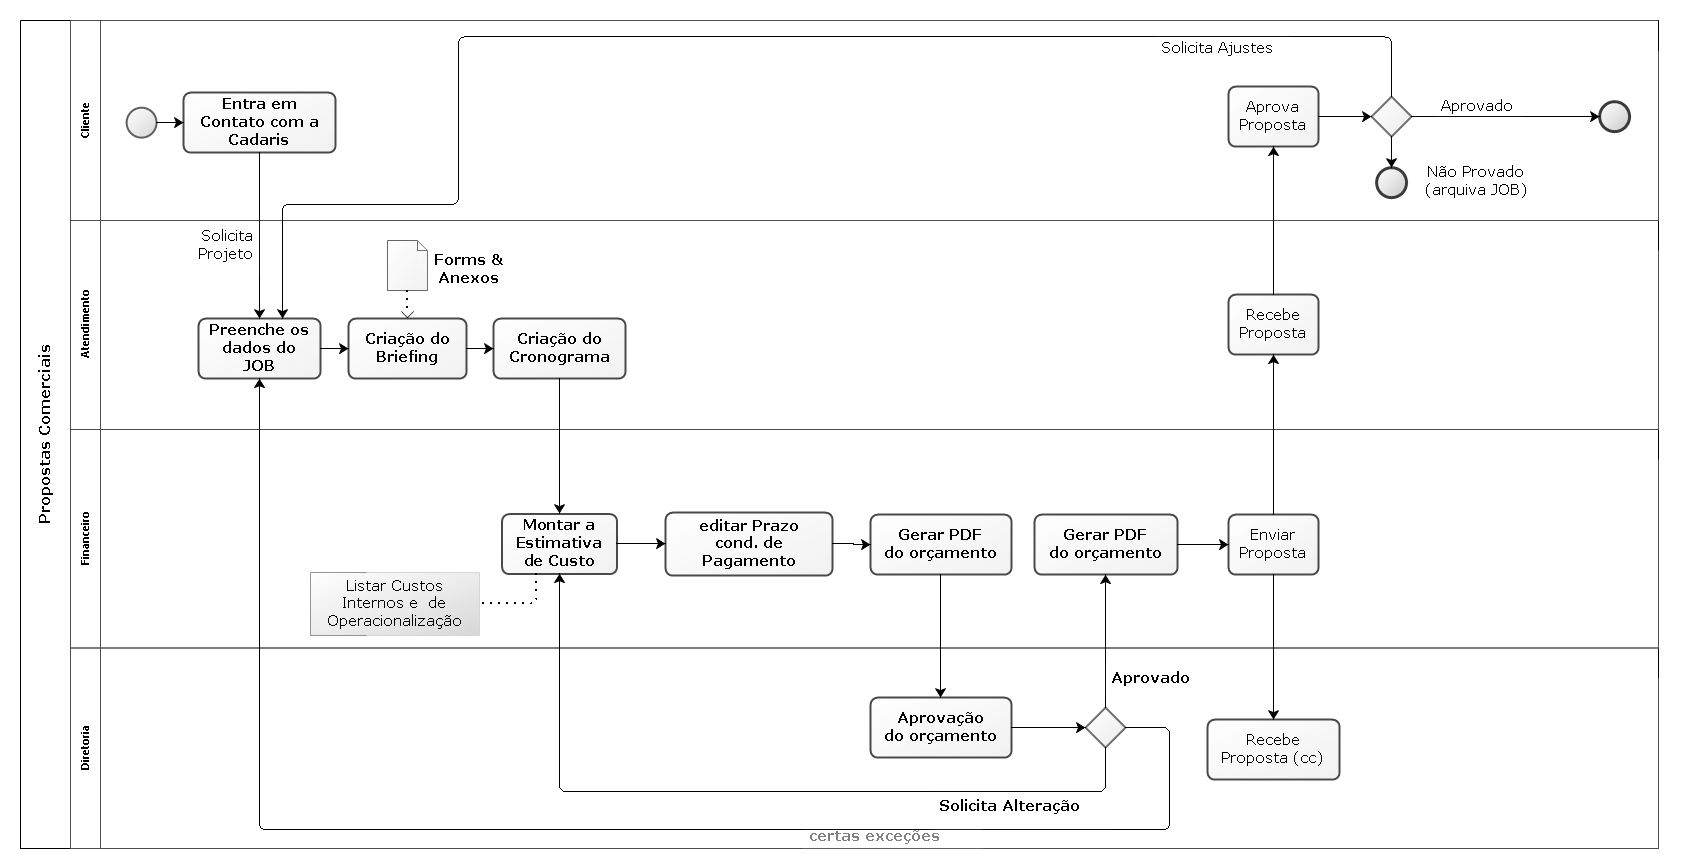
\includegraphics[width=\linewidth]{ModeloProcesso_Comercial_PeB}
  \caption{Modelo de Processo da Proposta Comercial}
  \label{fig:modProcess}
\end{figure}


A etapa de Produção do \textit{job} é realizado pelo setor de produção da Cadaris, utilizando técnicas e outras ferramentas especificas para o serviço desejado, como o \textit{Trello}\footnote{Ferramenta de gerenciamento de projetos em listas extremamente versátil, utilizando o método de \textit{Kanban} para indicar o andamento dos fluxos de produção.} para o gerenciamento do processo de produção. Concluido a produção do \textit{job}, o produto/serviço é entregue ao cliente. E para finalizar, o \textit{job} é encaminhado para o faturamento. 

Também há outras rotinas administrativas que este projeto pretende abranger, já que são realizadas em um processo não automatizado, com o auxílio de planilhas eletrônicas: 


{\singlespacing
\begin{itemize}
  \item Contas a receber;
  \item Contas a pagar;
  \item Controle RH:
  \begin{itemize}
    \item Folha de pagamento;
    \item Salário;
    \item Férias;
    \item Faltas/Atrasos;
    \item Folgas;
    \item Horas Extras;
    \item Vale Refeição;
    \item Vale Transporte;
  \end{itemize}
  \item Controle de Contratos;
  \item Cotação de Fornecedores;
  \item Relatórios:
  \begin{itemize}
    \item Relatório de Comissão;
    \item Relatório de Classificação de Receita;
    \item Relatório de Classificação de Despesa;
    \item Relatório Financeiro (Fluxo de Caixa);
  \end{itemize}
\end{itemize}
}


\subsubsection{PROBLEMAS ATUAIS E O PROJETO DE UM NOVO SISTEMA}

Para compor a Proposta Comercial, este sistema contratado apresenta muitos problemas pelo qual os funcionários devem enfrentar. Resultando em empecilhos para a boa usabilidade e atrapalhando a performance do funcionário. Nesta seção será apontado defeitos do sistema atual e melhorias de recursos necessárias que o novo sistema deverá ter.

O sistema atual tenta ser generalista para suportar inúmeras áreas da empresa e agências com regras de negócio distintas. Assim, muitos de seus módulos se tornam ineficientes para atuar nos novos modelos de negócio, com muitos campos redundantes, ou sem funcionalidade, e não conta com operações automatizas. Um dos problemas mais comuns e sérios que ocorrem é que elementos importantes tem sua relação baseada na inserção manual de códigos identificadores, para realizar a vinculação de um objeto a outro. Assim, de um ponto de vista da experiência do usuário, atrapalha a usabilidade do sistema e facilita o erro humano.

Para o preenchimento do \textit{Briefing}, além de um campo para a escrita livre, são necessários formulários especializados para os tipos de \textit{jobs} que a agência realiza, facilitando e padronizando a confecção destes \textit{Briefings}. O Cronograma é elaborado manualmente, então se faz necessário a incorporação de alguma ferramenta de simples utilização para a elaboração do cronograma estimado, pelo atendente, para a realização do \textit{job}.

Para a transferência do \textit{job} cadastrado de um departamento para outro, durante a passagem das etapas, no sistema atual é necessário realizar um \textit{PIT}\footnote{Abreviação para Pedido Interno de Trabalho, é um documento com todas as informações necessárias para solicitar a realização de algum trabalho.}, que é livre para enviar para qualquer pessoa. Mas, visto que a Proposta Comercial da Cadaris segue uma ordem pré-estabelecida de etapas e departamentos envolvidos, então a adoção de um sistema mais especializado é uma ótima solução para agilizar o processo e impedir possíveis erros.

Já para a elaboração da estimativa de custo, em vários quesitos o sistema não atende corretamente ao modelo de negócio da Cadaris. Uma estimativa de custo contempla Custos Internos e Custos de Operacionalização que por sua vez é composto por listas de itens com seus respectivos valores, e para a elaboração desta lista de custos, além de campos desnecessários, há a falta de certas funcionalidades, tais como: maior personalização de taxamentos, arredondamento de valor, subcategorias de Tipo de Serviço no Custo Interno, valores padrão para cada Tipo de Serviço e outras funcionalidades. 

O mais crítico do sistema é que essa estimativa de custo não é diretamente relacionada ao \textit{job}. Então, torna-se necessário preencher campos distintos com a mesma informação, pois o sistema não obtém esta informação do \textit{job} que deveria estar associado a ele. Algumas informações também importantes acabam sendo armazenadas em campos de observações por não ter campos próprios para aquela informação. E para finalizar, a estimativa não carrega as condições de pagamentos dos clientes, já que são distintas para cada um.

Ao final é gerado um documento em PDF contendo esta estimativa, porém faltam informações importantes neles como o prazo e condições de pagamento, e a lista de itens não são corretamente expostas. E no sistema atual este PDF da proposta pode ser gerado mesmo sem a aprovação da diretoria, havendo a necessidade de um bloqueio até a aprovação.

Durante todas estas etapas, é também utilizado no \textit{Trello} um \textit{card} para mostrar o estado do \textit{job}. Mostrando a necessidade de utilizar mais de uma ferramenta para gerenciar o processo de Proposta Comercial.

Para o gerenciamento de outros recursos, como: Funcionários, Departamentos, Clientes e Fornecedores, são utilizados planilhas eletrônicas. Sendo todo os processos relativos a estes recursos feito de modo não automatizado e sem uma centralização dos dados que são relacionados entre si.

Resumindo, a proposta geral deste projeto é o desenvolvimento de um sistema ERP\footnote{Abreviação em inglês para \textit{Enterprise Resource Planning}, ou seja, Planejamento dos Recursos da Empresa.}, que deve cuidar de todo o trabalho administrativo e operacional feito na Cadaris, e também automatizar todas estas tarefas antes feitas manualmente. Como por exemplo: faturamento, balanço contábil, fluxo de caixa, administração de pessoal, contas a receber, o dissídio, cálculo de férias e o ponto dos funcionários, e outros.

Há também um módulo especializado em atender a Proposta Comercial e todos os outros processos envolvidos nele.

Outros requisitos importantes são: o sistema deve ser de fácil acesso; possibilidade de utiliza-lo online e fora das dependências da empresa; garantir a disponibilidade; garantir a integridade, a segurança e a centralização de todos os dados; hierarquia de usuários; reduzir ao máximo o custo para desenvolvê-lo e mantê-lo ativo.



%  \noindent TODO: \\
%  - Explicar como eh o Comercial atual (VBD) OK \\
%  - dependeria de outros recursos (func client forn) q usa planilhas e códigos loucos OK \\
%  - automatizar tarefas/rotinas administrativas (ferias, horas, dissidio) OK \\
%  - producao (trello) OK \\
%  - finaceira (contas receber/pagar) OK \\
%  - integracao total dos dados, seguranca, divisao de usuarios e responsabilidades (hierarquia) OK \\




\subsection{ESTUDO DAS TECNOLOGIAS DE DESENVOLVIMENTO WEB}

Nesta subseção é relatada como ocorreu o estudo para a escolha de todas as tecnologias a serem empregadas no desenvolvimento deste sistema WEB, na qual muitas delas o aluno ainda não havia tido contato.

Como pode ser visto nas seções a diante, a UFABC oferece, por meio de disciplinas, todo o embasamento necessário para o desenvolvimento de um sistema, como: teoria da computação; concepção de um sistema de informação; modelamento de banco de dados; conceitos de interface gráfica; paradigmas de programação; programação para web e dispositivos móveis. 

O mercado de trabalho necessita e busca sempre por praticidade, seguindo tendências de desenvolvimento e utilizando o que há de mais novo e eficiente no mercado. Atualmente, há diversos métodos e padrões de projetos que garantem eficiência de uma implementação. Além de inúmeras linguagens de programação, na qual nelas a massiva adoção de \textit{frameworks} para diversos fins.

Um \textit{framework} é um conjunto (ou biblioteca) de classes que se relacionam entre si para disponibilizar ao desenvolvedor funcionalidade especificas. Basicamente um \textit{kit} de ferramentas devidamente implementada, testadas e prontas para o uso. Poupando assim, tempo e trabalho do desenvolvedor de implementar operações básicas como acesso a banco de dados, sistema de templates, mapeamento de rotas, autenticação de usuário e validação de dados.

Com todos os requisitos discutidos anteriormente, escolher corretamente como será formada a arquitetura do sistema foi de total importância. Escolher uma linguagem de programação e com ela um de seus \textit{frameworks} disponíveis, determinará os requisitos mínimos para sua execução, como os custos para desenvolvê-lo e mantê-lo, e viabilizará todos os recursos requisitados. E também é relevante saber seus limites e a possibilidade de utilizar outras bibliotecas para apoiar a necessidade, assim então garantir o sucesso da implementação deste sistema web.

De início foi escolhido a linguagem \textit{PHP}, que será melhor explicada nas seções seguintes, como a linguagem para o \textit{Back-end}, onde será executada em um servidor, afim de servir páginas dinâmicas de \textit{HTML} ao cliente em um navegador de internet. A escolha desta linguagem dar-se pelo fato do discente já ter familiaridade com o desenvolvimento web utilizando \textit{PHP}.

A tarefa seguinte era a pesquisa e escolha de um \textit{framework} para apoiar o desenvolvimento. Após a leitura de blogs e artigos na internet sobre os melhores \textit{frameworks PHP}~\cite{top10}. Após pequenos testes e exames de projetos exemplos que utilizam o \textit{framework}, foi decidido pelo aluno que o \textit{framework} será o \textbf{LARAVEL}. Eleito como o mais popular por diversos sites, como o Sitepoint~\cite{sitepoint}, o Laravel foi lançado em 2011, mas apesar de ser relativamente novo, tem um enorme ecossistema, com uma ótima documentação e conteúdo didático na internet.

Para o aprender a utilizar o Laravel, o aluno estudou através de vídeo-aulas gratuitas disponíveis na plataforma \textit{LARACASTS}~\cite{laracast} e sempre consultando a documentação oficial~\cite{laraveldocs} Obtendo assim aptidão para criar aplicações web utilizando este \textit{framework}, conhecendo suas funcionalidades e recursos disponíveis.

Para então iniciar a implementação deste sistema ERP.



%\subsection{DESENVOLVIMENTO DO SISTEMA} 

%  \subsubsection{CADASTROS}
  
%  \noindent TODO p/ estagio 1: \\
%  Funcionários \\
%  - CRUD \\
%  - Histórico do funcionário (admissão, promoção, ajuste VR/VT, férias)\\
%  - Histórico em Lote\\
%  - dissidio automático \\
%  - Relatório de faixa Salarial \\
%  - Relatório de férias \\
%  - Controle de Pontos (Atraso, Faltas(com Atestado), Folgas(Abonadas), Horas Extras) \\
%  Departamentos \\
%  Usuários \\
%  Clientes \\
%  - Empresa \\
%  - Departamento \\
%  - Centros de Custos \\
%  Fornecedores \\
%  - Empresa \\
%  - Centros de Custos 

  
%  \subsubsection{PROPOSTA COMERCIAL}
%  \noindent TODO p/ estagio 2: \\
%  - Listagem \\
%  - tipos de Create \\
%  - Briefing \\
%  - Cronograma \\
%  - Orçamento \\
%  - cond pgto \\
%  - PDFs \\
%  - Aprovação da Diretoria \\
%  - Aprovação do Cliente \\
%  - Produção
  
    
%  \subsubsection{RELATÓRIOS E CONTROLE FINANCEIRO}
%  \noindent TODO p/ estagio 3: \\
%  - Listagem \\
%  - tipos de Create \\
%  - Briefing \\
%  - Cronograma \\
%  - Orçamento \\
%  - cond pgto \\
%  - PDFs \\
%  - Aprovação da Diretoria \\
%  - Aprovação do Cliente \\
%  - Produção


%\subsection{INTERFACE E EXPERIÊNCIA DE USUÁRIO}
%  \noindent TODO p/ estagio 3: \\
%  Front-end


%\subsection{HOMOLOGAÇÃO, E AJUSTE FINAIS}

%\subsection{OUTRAS ÁREAS DA EMPRESA}

%\subsubsection{Resultados}
%\subsubsection{Conclusão}

%\subsection{DIAGNÓSTICO DOS PRINCIPAIS PROBLEMAS OBSERVADOS E SUGESTÕES DE MELHORIA}



\clearpage
\section{FUNDAMENTAÇÃO TEÓRICA}

%%-- Descrever as disciplinas utilizadas e dar exemplos--%%

Para a formação integral do discente é necessário que o conhecimento abordado nas disciplinas que foram cursadas se alinhe com a vivência prática do estágio, isto porque, necessita ser um processo de aprendizagem e profissionalização mútua do meio acadêmico e ambiente corporativo. 

A Tabela~\ref{tab:ementas} apresenta as disciplinas cursadas pelo aluno na Universidade Federal do ABC e que foram necessárias para o desenvolvimento das atividades do estágio. Nas subseções seguintes é descrito também quais foram as ferramentas utilizadas.

%   LISTA DE DISCIPLINAS E EMENTA
%  Algoritmo e estrutura de dados
%    Filas
%    Listas
%    Pilhas
%    Ordenação
%  
%  Análise de algoritmos
%    Custo de operações
%  
%  Banco de dados
%    Banco de dados relacional
%    Diagrama Entidade-Relacionamento
%    Diagrama de classes
%    Consultas SQL
%  
%  Bases Computacionais da Ciência
%    Planilhas
%  
%  Engenharia de software
%    Planejamento
%    Modelo Entidade-Relacionamento
%    Padrão MVC
%  
%  Interação Humano-Computador
%    Usabilidade
%    Padrões para interfaces
%    Técnicas de design
%    Ciclo de vida da engenharia de usabilidade
%    Métodos para avaliação da usabilidade
%  
%  Lógica básica
%    Operadores Lógicos
%  
%  Processamento da informação
%    Lógica de programação
%  
%  Programação orientada a objetos
%    Paradigma orientado a objetos
%  
%  Programação para Dispositivos Móveis
%    HTML
%    Responsividade
%  
%  Programação para Web
%    HTML
%    CSS
%    Javascript
%    Modelo MVC
%  
%  Segurança de Dados
%    Criptografia
%    Autenticação
%  
%  Sistemas de Informação
%    Desenvolvimento de sistemas de informação
%    Fundamentos de sistemas
%    Aplicações empresariais
%    ERP - Planejamento dos Recursos Empresariais



\begin{table}[!h] %[!htb]
\centering
\caption{Disciplinas cursadas com os suas respectivas abordagens praticadas no estágio.}
\label{tab:ementas}

\begin{tabular}{|c|l|}
  \hline
  
  Algoritmo e Estrutura de Dados                       
  &
  \begin{tabular}[c]{@{}l@{}}
    Filas \\
    Listas \\
    Pilhas \\
    Ordenação
  \end{tabular} \\ 
  \hline
  
  Análise de Algoritmos                       
  &
  Custo de operações \\ 
  \hline
  
  Banco de dados                       
  &
  \begin{tabular}[c]{@{}l@{}}
    Banco de Dados Relacional \\
    Diagrama Entidade-Relacionamento \\
    Diagrama de Classes \\
    Consultas SQL
  \end{tabular} \\ 
  \hline
  
  Engenharia de Software                       
  &
  \begin{tabular}[c]{@{}l@{}}
    Planejamento \\
    Modelo Entidade-Relacionamento \\
    Padrão MVC
  \end{tabular} \\ 
  \hline 
  
  Interação Humano-Computador                       
  &
  \begin{tabular}[c]{@{}l@{}}
    Usabilidade \\
    Técnicas de Design para Interfaces \\
    Ciclo de Vida da Eng. de Usabilidade \\
    Métodos para Avaliação da Usabilidade
  \end{tabular} \\ 
  \hline 
  
  Lógica Básica                   
  &
  Operadores Lógicos \\ 
  \hline 
  
  Processamento da informação                       
  &
  Lógica de programação \\ 
  \hline 
  
  Programação Orientada a Objetos                       
  &
  Paradigma Orientado a Objetos \\ 
  \hline 
  
  Programação para Dispositivos Móveis  
  &
  Responsividade  \\
  \hline 
  
  Programação para Web                       
  &
  \begin{tabular}[c]{@{}l@{}}
    HTML \\
    CSS \\
    Javascript \\
    Modelo MVC
  \end{tabular} \\ 
  \hline
  
  Segurança de Dados                       
  &
  \begin{tabular}[c]{@{}l@{}}
    Criptografia \\
    Autenticação
  \end{tabular} \\ 
  \hline
  
  Sistemas de Informação                       
  &
  \begin{tabular}[c]{@{}l@{}}
    Fundamentos de SI \\
    Aplicações Empresariais e ERP
  \end{tabular} \\ 
  \hline
  
\end{tabular}
\end{table}



\subsection{ENGENHARIA DE SOFTWARE E SISTEMAS DE INFORMAÇÃO}
Para garantir que um \textit{software} seja bem sucedido é necessário seguir determinadas especificações descritas pela Engenharia de Software, verificando assim qual iria atender melhor as necessidades dos usuários e os evitariam de futuras falhas.

Como descrito por Pressman~\cite{pressman}, ter o planejamento completo do projeto antes da própria implementação é extremamente importante. Com um bom planejamento, o sistema irá reduzir drasticamente o impacto de suas falhas, enquanto o \textit{software} estiver em larga utilização.

Diversas especificações foram abordadas na disciplina \textbf{Engenharia de software}, e o discente as colocou em prática ao desenvolver este sistema. Até nas reuniões iniciais na empresa as técnicas aprendidas em aula foram aplicadas com o apoio de diagramas e modelos para documentar o \textit{software} a ser implementado.

Conceitos importantes, sobre a aplicação de um \textit{software} para o apoio da regra de negócio de uma empresa, foram discutidos na disciplina \textbf{Sistemas de informação} e também aplicados neste projeto. Desta forma, idealizar e projetar uma ferramenta capaz de sanar as dificuldades atuais, substituir outras ferramentas defasadas e obter a centralização de todos os dados, se tornaram os objetivos primordiais para o desenvolvimento deste sistema ERP.

\subsection{DESENVOLVIMENTO WEB}
Como um dos principais requisitos do sistema é estar \textit{online}, criar um \textit{WebApp} pode ser considerado complexo, pois utilizam diferentes tecnologias para criar uma aplicação semelhante ao de \textit{desktop}, porém em um navegador de internet. Esta aplicação é executada em um servidor que receberá requisições do cliente e retornará respostas a ele conforme as ações desejadas. Enquanto no navegador, haverá a exibição das informações necessárias, além de suportar as interações do usuário. 

Pode-se então separar uma \textit{WebApp} em duas camadas: \textit{Back-end} e \textit{Front-end}. Em que o \textit{Front-end} é o responsável por interagir com o usuário, a fim de coletar os nados necessários e transmiti-los ao \textit{Back-end}, para que estes dados possam ser processados para retornar uma resposta.

Todos os fundamentos necessários foram apresentados durante a disciplina de \textbf{Programação para Web}. Como também outros fundamentos discutidos nas disciplinas de \textbf{Processamento da Informação}, \textbf{Programação Orientada a Objetos}, \textbf{Lógica Básica}, \textbf{Algoritmos e Estrutura de Dados} e \textbf{Análise de Algoritmos}. 

A disciplina de \textbf{Segurança de Dados} também contribuiu para os conceitos referentes à segurança de um sistema que foram necessários para o desenvolvimento deste projeto.

Nas subseções seguintes, será descrito as tecnologias utilizadas.

\subsubsection{BACK-END}
Do lado do servidor, sua principal função é receber requisições e devolver respostas. Além de ter acesso ao banco de dados e realizar todo o processamento dos dados necessários.

\subsubsubsection{PHP}
O PHP\footnote{PHP é um acrônimo recursivo para \textit{PHP: Hypertext Preprocessor}, originalmente \textit{Personal Home Page}.} é uma linguagem interpretada capaz de gerar uma página web a ser visualizada no lado do cliente. Suas principais características são sua velocidade e robustez, orientada a objetos, independente de plataforma e tipagem dinâmica. 

Há várias extensões que possibilita o PHP se conectar com outras ferramentas, como: inúmeros Bancos de Dados, \textit{socket}, geração de PDF, OpenSLL e outros. Por isto, foi considerada a melhor escolha para ser utilizada no \textit{Back-end}, principalmente por ser gratuita sua utilização, diminuindo assim, os custos para o desenvolvimento e execução do sistema.



\subsubsubsection{LARAVEL}
Laravel é um \textit{framework} PHP livre e \textit{open-source} para o desenvolvimento de sistemas web, utilizando o padrão MVC\footnote{Abreviação para \textit{Model-view-controller}, em português modelo-visão-controlador, é um padrão de arquitetura de software que separa em camadas, cada uma com suas responsabilidades.}. O Laravel possui recursos e características que sobressaem dos demais \textit{framework}, como: 

{\singlespacing
\begin{itemize}
  \item Sua sintaxe simples e concisa;
  \item Um sistema modular com gerenciador de dependências dedicado;
  \item Várias formas de acesso a banco de dados relacionais;
  \item Vários utilitários indispensáveis no auxílio ao desenvolvimento e manutenção de sistemas;
  \item \textit{Eloquent ORM} para mapeamento objeto-relacional;
  \item \textit{Query Builder} é um conjunto de classes e métodos capaz de criar consultas em banco de dados em forma de programação;
  \item Roteamento de links;
  \item Controladores \textit{Restful};
  \item Carregamento automático de classes sob demanda;
  \item Compositores de \textit{View}, como o \textit{Blade}, para compor a visão e fornecer estruturas de controle e utiliza o cache para melhor desempenho;
  \item \textit{Database Migration} para versionar a estrutura do banco de dados, facilitando o desenvolvimento e a manutenção do sistema;
  \item \textit{Database seeding} para popular o banco de dado com dados a serem utilizados em testes.
  \item Paginação automática nas listagens de dados;
  \item \textit{Form request} para validação da entrada de dados vindo do cliente;
  \item \textit{Artisan CLI} é uma interface de linha de comandos para automatizar tarefas, como a migração do banco de dados ou criação de componentes do Laravel, ajudando a melhor gerir o projeto no \textit{framework};
  \item Código fonte do Laravel está hospedado no GitHub;
  \item Licença MIT.
\end{itemize}
}

\subsubsubsection{BANCO DE DADOS}

Banco de dado é o conjunto organizado de dados que se relacionam entre si, desta forma, permite que informações importantes sejam armazenadas. 

Os Banco de Dados são operados por um SGBD\footnote{Abreviação para Sistema Gerenciador de Banco de Dados.}, este gerenciador disponibiliza uma interface para que os clientes possam incluir, alterar ou consultar dados previamente armazenados. Em bancos de dados relacionais, esta interface é constituída por um driver do SGBD que executam comandos na linguagem SQL\footnote{Abreviação de \textit{Structured Query Language}, ou me português, Linguagem de Consulta Estruturada}

O SGBD utilizado no sistema foi o MySQL e a disciplina \textbf{Banco de Dados} instruiu em como desenvolver a uma estrutura sólida e coerente conforme as formas normais.

Para se conectar ao MySQl, o Laravel torna a interação com o banco de dados simples, utilizando o \textit{fluent query builder} e o Eloquent ORM como interfaces para o desenvolvedor ter acesso ao banco de dados.


% TODO: exemplo de consulta com Laravel - Eloquent ORM



\subsubsection{FRONT-END}
O \textit{Front-end} é o lado do cliente, no qual fornece uma interface amigável para o usuário, a fim de exibir dados e coletar informações vindas da interação do usuário com o sistema.

Em relação à interface do usuário foi necessário a aplicação de conceitos discutidos na disciplina \textbf{Interação Humano-Computador} que foi abordado os conceitos fundamentais para criar uma interface com melhor acessibilidade e usabilidade nas suas funcionalidades, para garantir uma melhor experiência de uso pelo usuário.

Para desenvolver esta interface, são utilizadas diversas ferramentas, e as principais serão apresentados a seguir.


\subsubsubsection{HTML}
O HTML\footnote{Abreviação para \textit{Hyper Text Markup Language}, ou seja, Linguagem de Marcação de Hipertexto em português.} é uma linguagem de marcação base da estrutura da interface de uma página na internet. A última versão é o HTML5 e foi publicada em 28 de outubro de 2014, toda a especificação do HTML é padronizado pelo W3C~\cite{w3c}.
Na codificação de um documento, o HTML possui marcadores, chamadas \textit{tags}, entre os caracteres \texttt{<} e \texttt{>}. Um elemento do HTML é formado por uma \textit{tag} com seus atributos e valores, e como descendente pode-se haver outros elementos ou textos. Esta estrutura será interpretada pelo navegador para compor elementos a serem renderizados e exibidos ao usuário.


% TODO: exemplos de estruturas...


\subsubsubsection{CSS}
O CSS\footnote{Abreviação de \textit{Cascading Style Sheets}.} é uma linguagem de folhas de estilo que serve para definir a aparência dos elementos no HTML a serem renderizados na interface, como: cor, altura, largura, fonte de textos, sombras e etc.

% TODO: exemplos de Sintaxe e Seletores...

% TODO: BootStrap3 


\subsubsubsection{JAVASCRIPT}
O JavaScript é uma linguagem interpretada pelo navegador para executar \textit{scripts} do lado do cliente ao invés de somente do servidor, possibilitando controlar elementos da página dinamicamente, com execução e comunicação assíncrona. É uma linguagem orientada a objetos baseada em protótipos, tipagem fraca e dinâmica, funções de primeira classe e possui suporte a programação funcional.

Por meio do AJAX\footnote{Abreviação para \textit{asynchronous JavaScript and XML}, em português, Javascript e XML Assíncrono.}, o JavaScript pode se comunicar com o servidor de modo assíncrono, podendo  enviar dados do cliente e obter dados do servidor. Mas normalmente, utiliza-se JSON ao invés de XML para transportar os dados em AJAX.

O JSON\footnote{Acrônimo para \textit{JavaScript Object Notation, ou em português, Notação de Objeto de JavaScript}.} é um formato mais leve que o XML para trocas de dados. Amplamente utilizado em sistemas que fluxo de dados entre o cliente e o servidor é vital para o sistema.

Também foi utilizada a mais popular biblioteca de funções JavaScript, chamada jQuery, que ajuda simplificando: a interação com o HTML, a seleção de elementos na DOM, criar animações, manipular eventos, realizar chamadas AJAX e a criação e utilização de \textit{plugins}. Permitindo criar uma camada de abstração que simplifica o desenvolvimento de aplicações web.




\clearpage
\section{CONSIDERAÇÕES FINAIS}
%%-- Conclusão do relatório, enfatizar os resultados a contribuição para a formação, dificuldades e futuras melhoras --%%


Este capítulo tem como objetivo descrever as contribuições que o estágio proporcionou à formação acadêmica e profissional, incluindo as dificuldades encontradas durante o processo e sugestões de futuros trabalhos.


\subsection{CONTRIBUIÇÕES PARA A FORMAÇÃO}

Foi necessário o conhecimento e aplicação de algumas disciplinas cursadas para a realização do estágio, sendo elas: Algoritmo e Estrutura de Dados; Análise de Algoritmos; Banco de Dados; Bases Computacionais da Ciência; Engenharia de Software; Interação Humano-Computador; Lógica Básica; Processamento da Informação; Programação Orientada a Objetos; Programação para Dispositivos Móveis; Programação para Web; Segurança de Dados e Sistemas de Informação.

O estágio exigiu habilidades para resolução de problemas e conhecimentos técnicos em operadores lógicos; consultas em banco de dados; desenvolvimento de sistema de informação; desenvolvimento em camadas (MVC).

As ferramentas estudadas pelo discente nas disciplinas contribuíram para a facilidade do desenvolvimento do estágio, mas também alguns assuntos abordados foram aplicados em menor proporção nas atividades, enquanto outros foram necessários um aprimoramento mais aprofundado, considerando que o aprendizado em um ambiente acadêmico acontece em um cenário ideal e pequeno em relação ao mercado de trabalho.

O período total do estágio foi suficiente para perceber a diferença entre a teoria e a prática. Na teoria todo o assunto é passado ao discente, os conceitos, maneiras de resoluções de problemas, os exercícios e projetos são grandes desafios e são os que colocam à prova de tudo o que foi aprendido nas aulas. Porém, quando o aluno se depara com a realidade do mercado de trabalho, nota a diferença do que foi visto nas aulas teóricas, apesar de aparentar um projeto grande, é apenas um pequeno exemplo que pode acontecer no dia a dia do trabalho. Esse alinhamento entre a teoria e a prática faz com o que o discente amadureça os conhecimentos teóricos obtidos na sala de aula e os apliques em situações reais contribuindo no crescimento profissional.



\subsection{DIFICULDADES ENCONTRADAS}

O desenvolvimento de aplicações no ambiente de produção exige muita disciplina do profissional. O código deve ser bem estruturado, pois será mantido por uma equipe. Deve haver um planejamento do projeto antes de iniciar qualquer programação para evitar erros e trabalhos desnecessários. O profissional necessita pesquisar muito sobre como realizar a tarefa, e analisar qual seria a melhor solução, quais seriam as melhores ferramentas, conversar com outros desenvolvedores para adquirir experiência e criar uma solução ideal para o problema.

Algumas ferramentas utilizadas no decorrer do estágio não foram ensinadas nos cursos de formação do aluno, como os \textit{frameworks}, dificultando inicialmente o desenvolvimento dos projetos. Porém, tal fato implicou em um maior empenho e dedicação em estudos e pesquisas, gerando ótimos resultados nos projetos e amadurecendo o aluno profissionalmente.


\subsection{SUGESTÕES DE TRABALHOS FUTUROS}

As disciplinas ministradas aos alunos devem possuir uma reciclagem periodicamente, pois a área de tecnologia possui novidades constantemente. Além da reciclagem nos assuntos de cada disciplina, também é preciso verificar a necessidade de novas disciplinas que possam abranger as novidades de hardware e/ou software.

Os projetos desenvolvidos pelo aluno possuem tecnologias e ferramentas recentes e esse caminho deve ser mantido. Foram utilizadas ferramentas de código aberto que facilita a atualização por parte dos desenvolvedores e da comunidade que participa com constantes contribuições. Outras ferramentas e recursos podem ser agregados aos sistemas para facilitar a experiência do usuário, mas com cuidado para que não haja exageros e conflitos com as ferramentas atuais.

O Laravel demonstrou ser uma ferramenta com uma curva de aprendizado menor que as outras do mercado, porém o Laravel desempenha um grande papel no sistema, assim pode manter e aperfeiçoar o projeto para futuras melhorias se necessário


\clearpage
%\section{REFERÊNCIAS BIBLIOGRAFICAS}
\bibliographystyle{abbrv}
\bibliography{relEstagio1}

\end{document}
